\section{Project: Person mask detector model for edge devices}
\subsection{Motivation}

\subsection{Project scope}
Community analytics, an essential task in network analysis, involves the identification of groups or communities within a network structure. Two primary types of methods are commonly employed for community detection: agglomerative methods and divisive methods.
\begin{center}
    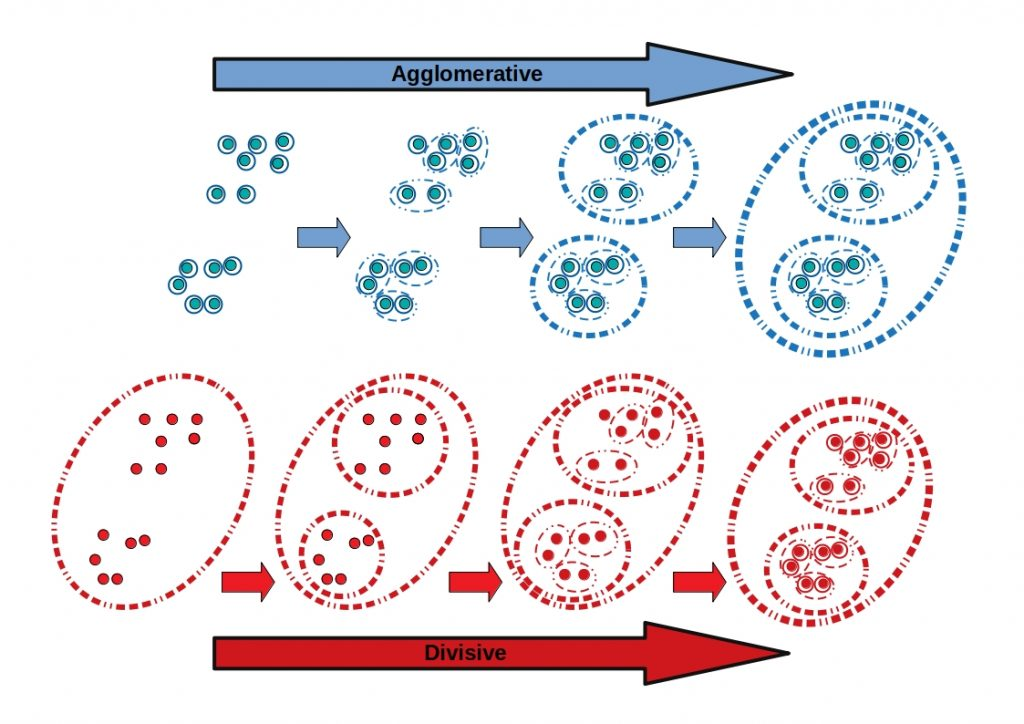
\includegraphics[scale=0.45]{image/agglo_divi_algo.jpeg}
\end{center}
In agglomerative methods (illustrated on the upper Figure 1), the process initiates with individual nodes and gradually merges them based on their similarity or connectivity, leading to hierarchical clustering. 

This approach merges nodes from the bottom up, progressively forming larger communities. The agglomerative category includes algorithms such as Louvain and Leiden, which utilize modularity and hierarchical clustering. 

Modularity, represented as Q, measures community strength and guides the algorithm. Higher modularity values indicate better communities, while a value below 1 suggests that each node is treated as a separate community. 

The dendrogram in Figure 1 represents the hierarchy of clusters generated by hierarchical clustering. On the other hand, divisive methods (depicted on the bottom of Figure 1) start with a single partition containing all nodes and iteratively split it by removing edges with low similarity. 

This process, known as the split process, aims to find smaller, more cohesive communities by progressively dividing the network. Although agglomerative and divisive methods employ different approaches, both ultimately aim to unveil meaningful groups of nodes based on their connectivity patterns within the network.

\subsection{Clauset-Newman-Moore greedy modularity maximization}
The Clauset-Newman-Moore (CNM) greedy modularity maximization algorithm is a popular method used in community detection, a field of network analysis. It is designed to partition a given network into communities, where members of each community are more densely connected to each other compared to members of different communities. The CNM algorithm aims to maximize the modularity of the network, which is a measure of the quality of the community structure.

The algorithm was proposed by Aaron Clauset, Mark Newman, and Cristopher Moore in 2004, and it has since become widely adopted due to its simplicity and effectiveness. The CNM algorithm is agglomerative method and follows a greedy approach, iteratively merging and splitting communities to optimize the modularity score.
\linebreak
\textbf{Network representation: } Considering an undirected network/graph with N nodes and E edges. We can represent the network as a graph adjacency matrix A of size N x N, where A[i][j] = 1 if there is an edge between nodes i and j, and A[i][j] = 0 otherwise.

A_{vw} = \begin{cases}
    1, & \text{if vertices } v \text{ and } w \text{ are connected}, \\
    0, & \text{otherwise}. \end{cases}


\linebreak
\textbf{Community Structure: } We represent the community structure of the network using a partition vector s of length N, where s[i] denotes the community membership of node i. Each node belongs to exactly one community.

The fraction of edges that fall within communities is given by:

\[
\frac{1}{2m} \sum_{vw} A_{vw} \delta(c_v, c_w)
\]

where:

- \(\sum_{vw} A_{vw}\) represents the summation over all pairs of vertices v and w, considering the elements of the adjacency matrix A. It computes the total number of edges in the graph, denoted as m.

- \(\delta(c_v, c_w)\) is the Kronecker delta function, which takes the value 1 if the community assignments of vertices v and w (cv and cw, respectively) are the same, and 0 otherwise.

- \(\frac{1}{2m}\) is a normalization factor, dividing by the total number of edges to ensure the measure falls within the range [0, 1].

However, this measure alone is not sufficient to evaluate the quality of a community structure. It reaches its maximum value of 1 in the trivial case where all vertices belong to a single community. Additional measures like modularity is considered for a comprehensive assessment of community structure.

\textbf{Modularity: } The probability of an edge existing between vertices v and w, assuming random connections while respecting vertex degrees, is given by \( \frac{k_v k_w}{2m} \). Here, \( k_v \) represents the degree of vertex v, \( k_w \) represents the degree of vertex w, and m is the total number of edges in the graph.

Based on this probability, we define the modularity Q as follows:
\begin{equation}
    Q = \sum_{s=1}_m\Big[\frac{l_s}{L}-\Big(\frac{d_s}{2L}\Big)^2\Big]
\end{equation}
(m = number of modules, ls = the number of edges inside module s, L = the number of edges in the network, dₛ = total degree of the nodes in module s)\\

This process of removing an edge and calculating the modularity is iteratively repeated. The algorithm will stop when the new modularity is no longer greater than the modularity from the previous iteration. The ending modularity is usually around 0.6.

\subsubsection{Pseudo Code}
\begin{algorithm}[H]
\caption{Clauset-Newman-Moore (CNM) Algorithm}
\SetAlgoLined
\KwIn{Network graph}
\KwOut{Community structure}
Initialization: Assign each vertex to its own community\;

Calculate the initial modularity value \( Q_{\text{initial}} \)\;

\Repeat{no further improvement in modularity is possible}{
        \ForEach{pair of communities \( C_1 \) and \( C_2 \)}{
            Calculate the change in modularity \( \Delta Q \) by merging \( C_1 \) and \( C_2 \)\;
        }
    }

Find the pair \( (C_1, C_2) \) with the maximum increase in modularity \( \Delta Q_{\text{max}} \)\;

Merge communities \( C_1 \) and \( C_2 \)\;
Update the modularity value \( Q \) by adding \( \Delta Q_{\text{max}} \)\;
\Return{Community structure}
\end{algorithm}

\subsubsection{Complexity}
Since the joining of a pair of communities between which there are no edges at all can never result in an increase in Q, we need only consider those pairs between which there are edges, of which there will at any time be at most m, where m is again the number of edges in the graph. 

The change in Q upon joining two communities is given by $\Delta Q = e_{ij} + e_{ji} - 2a_{i}a_{j} = 2(e_{ij} - a_{i}a_{j})$, which can clearly be calculated in constant time. 
Following a join, some of the matrix elements $e_{ij}$ must be updated by adding together the rows and columns corresponding to the joined communities, which takes worst-case time $O(n)$. Thus each step of the algorithm takes worst-case time $O(m + n)$. 

There are a maximum of $n - 1$ join operations necessary to construct the complete dendrogram and hence the entire algorithm runs in time $O((m + n)n)$, or $O(n^{2})$ on a sparse graph. The algorithm has the added advantage of calculating the value of $Q$ as it goes along, making it especially simple to find the optimal community structure.\\
Each step: worst-case time $O(m + n)$.\\
A maximum of $(n - 1)$ steps to join $n$ communities.\\
Thus: $O((m + n)n)$ or $O(n^{2})$ for sparse graphs.

\pagebreak
\subsubsection{Pros and Cons}
\paragraph{Pros}
\begin{itemize}
    \item Ease of implementation: Modularity Maximization (MM) is conceptually simple and can be implemented with relative ease compared to other algorithms. Several open-source libraries and software packages readily implement MM, making it accessible to a wide range of users.
    \item Scalability: MM efficiently scales to handle large networks with millions of nodes and edges. This makes it suitable for analyzing real-world networks like social media graphs, citation networks, and protein-protein interaction networks.
\end{itemize}
\paragraph{Cons}
\begin{itemize}
    \item Resolution limit: MM is sensitive to the resolution parameter, which controls the granularity of the detected communities. Choosing an appropriate resolution parameter can be challenging, as it can significantly impact the community structure. Small values tend to result in many small communities, while large values lead to a few large communities, potentially missing finer-grained structures.
    \item Merging similar clusters: MM can be biased towards merging similar clusters, even if they are not well-connected, to maximize the modularity score. This can lead to communities that are not cohesive or representative of the underlying network structure.
\end{itemize}

\subsection{Louvain Algorithm}
The Louvain algorithm is a widely used community detection algorithm that aims to identify communities or clusters within a network graph. It was developed by Vincent D. Blondel, Jean-Loup Guillaume, Renaud Lambiotte, and Etienne Lefebvre in 2008.

The algorithm is known for its efficiency and ability to handle large-scale networks. It follows a greedy optimization approach that iteratively improves the modularity measure of the network by merging and rearranging communities. 
It can be used to analyze a network of 2 million nodes in only 2 minutes \\
\begin{center}
    \begin{figure}[!htp]
    \centering
    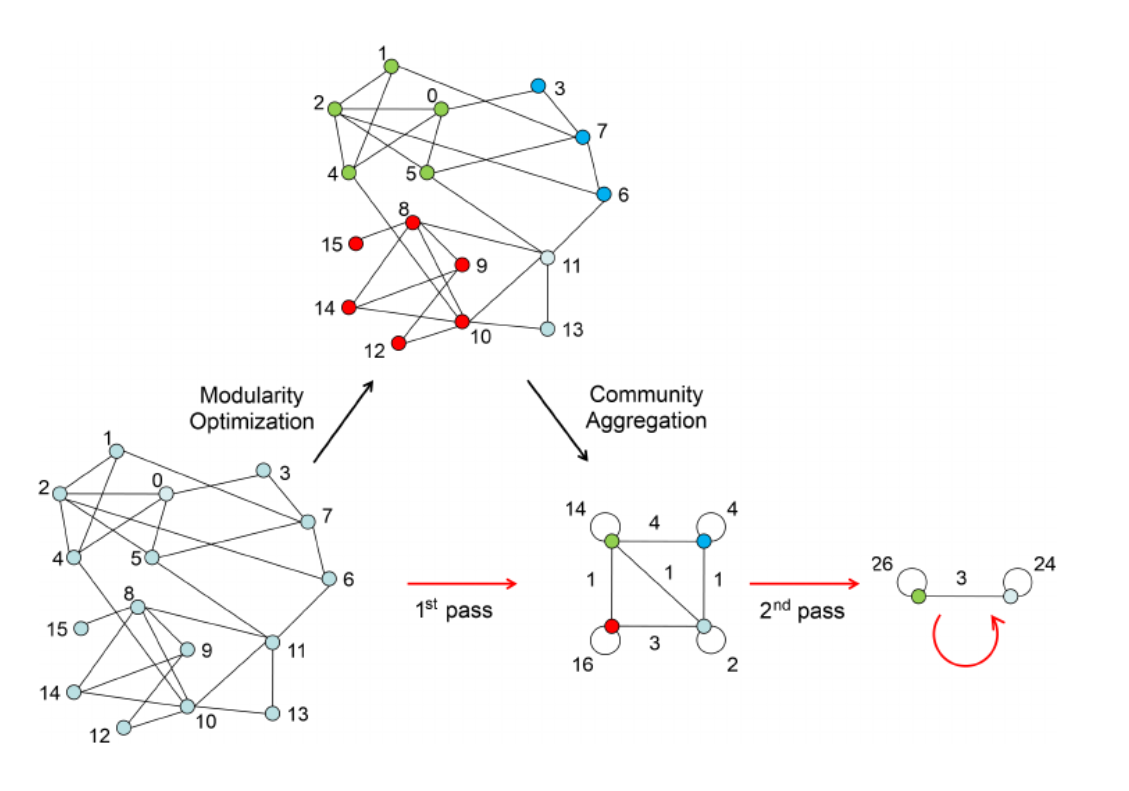
\includegraphics[width=0.7 \textwidth]{image/Louvain.png}
    \caption{Louvain Algorithm}
    \label{subsection}
\end{figure}
\end{center}
\subsubsection{Modularity Optimization}
As depicted in the figure, the first step is to optimize the modularity of the entire graph. In this example, it splits the nodes into four communities.

To find these clusters, each node is moved into its neighboring community. If the change in modularity (\(\Delta Q\)) is greater than 0, it is moved into the neighboring community. Otherwise, it remains in its current community. This process is repeated until \(\Delta Q = 0\) for all nodes.
\subsubsection{Community Aggregation}
After the optimization of modularity, super nodes are introduced to represent each cluster. Following the initial phase of the algorithm, numerous communities are formed.

Nevertheless, the two phases continue to iterate, resulting in the formation of larger and larger communities. The algorithm terminates only when neither of the two operations can further enhance the community structure.

\subsubsection{Pseudo Code}
\begin{algorithm}[H]
\SetAlgoLined
\KwIn{Graph $G=(V, E)$}
\KwOut{Community structure of the graph}
Initialize each node as a separate community\;

\Repeat{No further improvement in modularity}{
    \For{each node $v \in V$}{
        Remove $v$ from its current community\;

        Calculate the modularity gain $\Delta Q$ for each neighboring community by moving $v$\;
        
        Move $v$ to the neighboring community with the highest $\Delta Q$\;
    }
    Construct the aggregated network where each community is represented by a node\;
    
    Update the original graph with the new community assignments\;
}
\caption{Louvain Algorithm}
\end{algorithm}

\subsubsection{Pros and Cons}

Pros of the Louvain algorithm:
\begin{itemize}
    \item Fast and scalable for large networks.
    \item Optimizes modularity, which measures community quality.
    \item Detects hierarchical community structures.
    \item Allows flexibility in resolution for different levels of detail.
    \item Widely used with extensive resources and documentation.
\end{itemize}

Cons of the Louvain algorithm:
\begin{itemize}
    \item Resolution limit may merge small communities into larger ones.
    \item Results can be sensitive to initial community assignments.
    \item Assumes non-overlapping communities.
    \item Bias towards detecting large, cohesive communities.
    \item Lacks theoretical guarantees of optimality.
\end{itemize}


\subsection{Label Propagation Algorithm}
\subsubsection{Intuition}
As we will show, the advantage of this algorithm over the other methods is its simplicity and time efficiency. The algorithm uses the network structure to guide its progress and does not optimize any specific chosen measure of community strengths.
\subsubsection{Pseudocode}
\begin{enumerate}
    \item Initialize the labels at all nodes in the network. For a given node $x$, $C_{x}(0) = x$.
    \item Initialize $t = 1$.
    \item Arrange the nodes in the network in a random order and set it to $X$.
    \item For each $x$ in $X$ chosen in that specific order,\\
         let $C_{x}(t) = f(C_{x_{i1}}(t),\ldots,C_{x_{im}}(t),C_{x_{i(m+1)}}(t-1),\ldots,C_{x_{ik}}(t-1))$.\\
         $f$ here returns the label occurring with the highest frequency among neighbors and ties are broken uniformly randomly.
    \item If every node has a label that the maximum number of their neighbors have, then stop the algorithm. Else, increment $t$ and go to 3.
\end{enumerate}
\subsubsection{Complexity}
It takes a near-linear time for the algorithm to run to its completion Initializing every node with unique labels requires $O(n)$ time. Each iteration of the label propagation algorithm takes linear time in the number of edges $O(m)$.\\
At each node $x$, we first group the neighbors according to their labels $O(d_{x})$. We then pick the group of maximum size and assign its label to $x$, requiring a worst-case time of $O(d_{x})$. This process is repeated at all nodes and hence an overall time is $O(m)$ for each iteration.
\subsubsection{Pros and Cons}
\paragraph{Pros}
\begin{itemize}
    \item Efficiency: Label propagation is computationally efficient, making it suitable for large networks. Its running time is generally faster compared to some other community detection algorithms.
    \item Low A Priori Information Requirement: One of its notable strengths is its low dependency on prior information about the network structure. You don't need to specify parameters beforehand, which can be advantageous in scenarios where the network characteristics are not well-known.
\end{itemize}
\paragraph{Cons}
\begin{itemize}
    \item Lack of Unique Solutions: As you mentioned, the algorithm doesn't guarantee a unique solution. This can be a drawback if you're looking for a single, definitive community structure. The results can vary across different runs of the algorithm.
    \item Aggregate Solutions: The algorithm provides an aggregate of multiple solutions, leading to a lack of specificity. This might be undesirable in situations where a precise and unique community structure is crucial.
\end{itemize}
